\begin{figure}[ht!]
    \begin{subfigure}{.5\textwidth}
    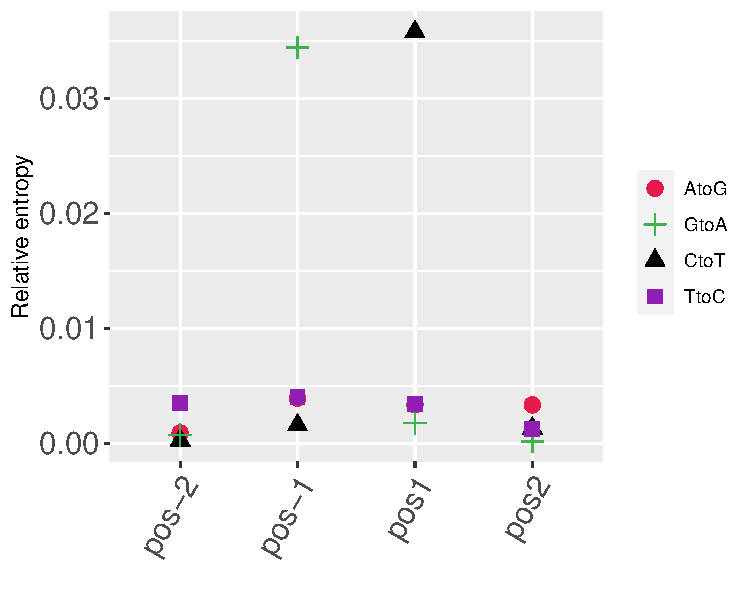
\includegraphics[scale=0.63]{graphics/nbr_transitions_Bone-Osteosarc.pdf}
    \caption{transitions/Bone-Osteosarc}
    \label{fig:transitions_bone-osteosarc}
    \end{subfigure}
    ~
    \begin{subfigure}{.5\textwidth}
    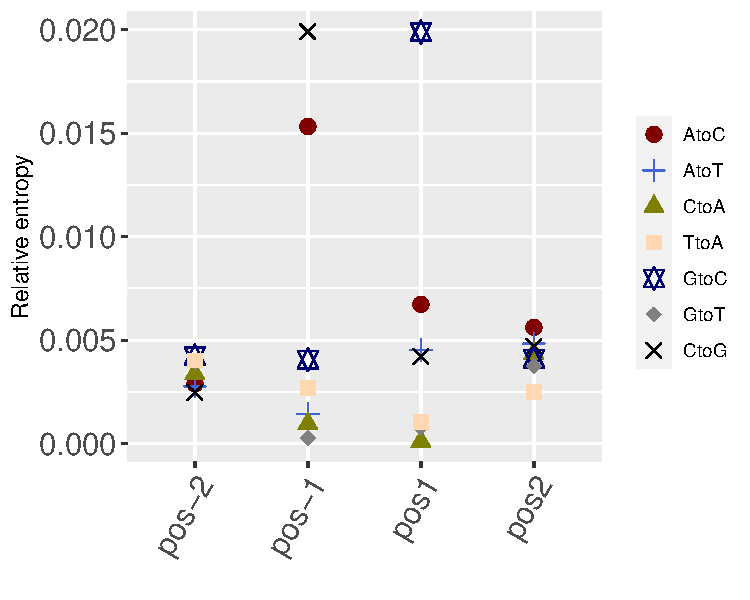
\includegraphics[scale=0.63]{graphics/nbr_transversion_Bone-Osteosarc.pdf}
    \caption{transversions/Bone-Osteosarc}
    \label{fig:transversions_bone-osteosarc}
    \end{subfigure} \\
    \vspace{0.5cm}
    
    \begin{subfigure}{.5\textwidth}
    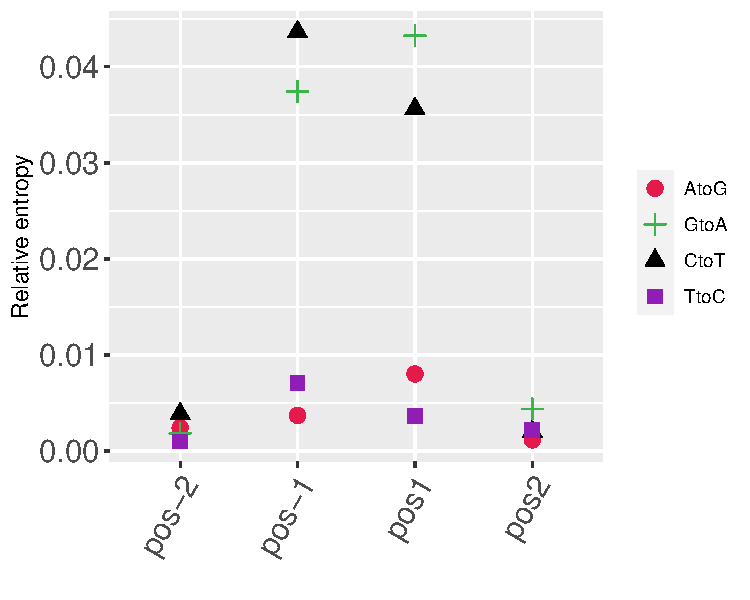
\includegraphics[scale=0.63]{graphics/nbr_transitions_Breast-AdenoCa.pdf}
    \caption{transitions/Breast-AdenoCa}
    \label{fig:transitions_breast-adenoca}
    \end{subfigure}
    ~
    \begin{subfigure}{.5\textwidth}
    \includegraphics[scale=0.63]{graphics/nbr_transversion_Breast-AdenoCa.pdf}
    \caption{transversion/Breast-AdenoCa}
    \label{fig:transversion_breast-adenoca}
    \end{subfigure} \\
    \vspace{0.5cm}
    
    \begin{subfigure}{.5\textwidth}
    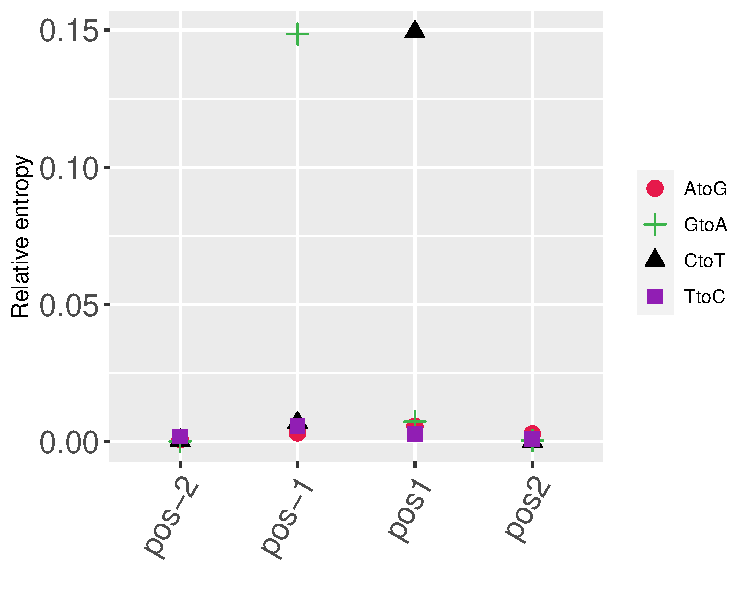
\includegraphics[scale=0.63]{graphics/nbr_transitions_CNS-Medullo.pdf}
    \caption{transitions/CNS-Medullo}
    \label{fig:transitions_cns-medullo}
    \end{subfigure}
    ~
    \begin{subfigure}{.5\textwidth}
    \includegraphics[scale=0.63]{graphics/nbr_transversion_CNS-Medullo.pdf}
    \caption{transversion/CNS-Medullo}
    \label{fig:transversion_cns-medullo}
    \end{subfigure} \\
    \caption{\textbf{Flanking bases are a good source of information.} Continued on next page.}
\end{figure}
\begin{figure}[ht!]\ContinuedFloat
    \begin{subfigure}{.5\textwidth}
    \includegraphics[scale=0.63]{graphics/nbr_transitions_CNS-PiloAstro.pdf}
    \caption{transitions/CNS-PiloAstro}
    \label{fig:transitions_cns-piloastro}
    \end{subfigure}
    ~
    \begin{subfigure}{.5\textwidth}
    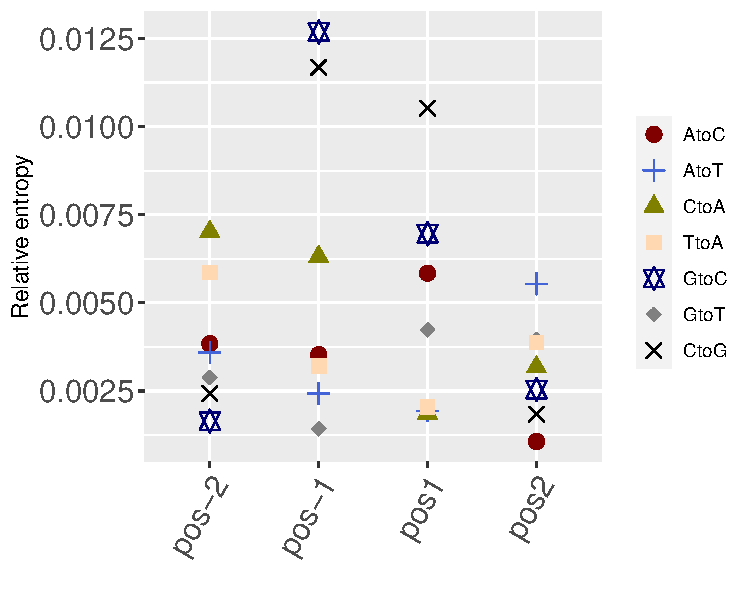
\includegraphics[scale=0.63]{graphics/nbr_transversion_CNS-PiloAstro.pdf}
    \caption{transversions/CNS-PiloAstro}
    \label{fig:transversions_cns-piloastro}
    \end{subfigure} \\
    \vspace{0.5cm}
    
    \begin{subfigure}{.5\textwidth}
    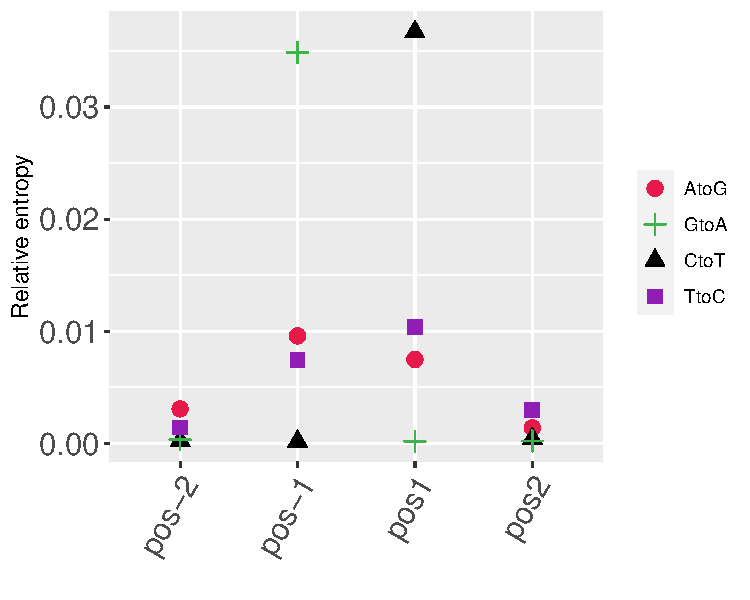
\includegraphics[scale=0.63]{graphics/nbr_transitions_Kidney-RCC.pdf}
    \caption{transitions/Kidney-RCC}
    \label{fig:transitions_kidney-rcc}
    \end{subfigure}
    ~
    \begin{subfigure}{.5\textwidth}
    \includegraphics[scale=0.63]{graphics/nbr_transversion_Kidney-RCC.pdf}
    \caption{transversion/Kidney-RCC}
    \label{fig:transversion_kidney-rcc}
    \end{subfigure} \\
    
    \begin{subfigure}{.5\textwidth}
    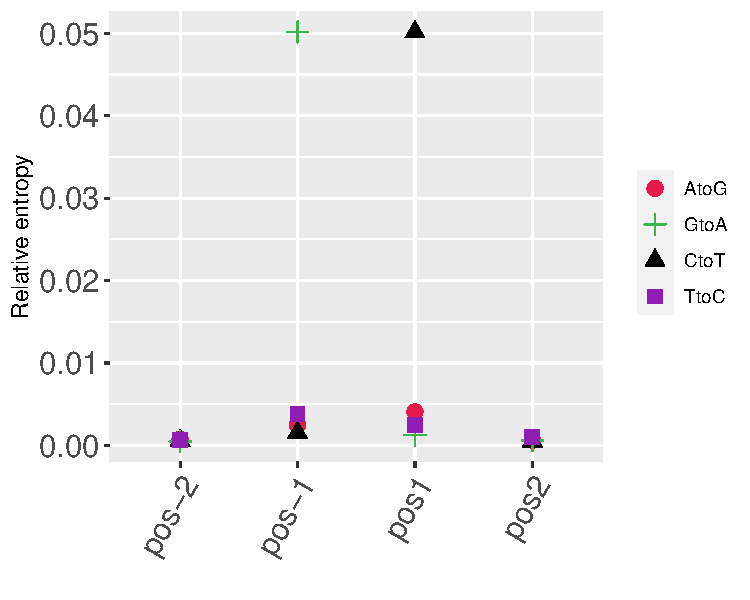
\includegraphics[scale=0.63]{graphics/nbr_transitions_Lymph-BNHL.pdf}
    \caption{transitions/Lymph-BNHL}
    \label{fig:transitions_lymph-bnhl}
    \end{subfigure}
    ~
    \begin{subfigure}{.5\textwidth}
    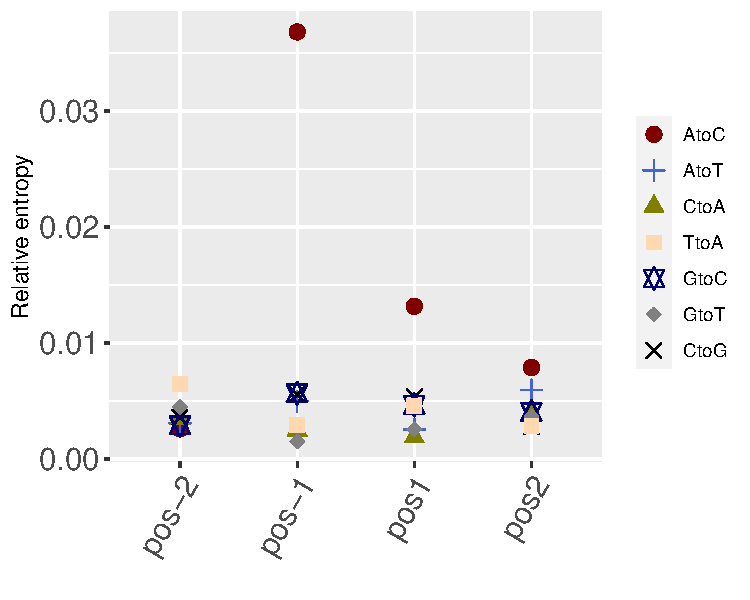
\includegraphics[scale=0.63]{graphics/nbr_transversion_Lymph-BNHL.pdf}
    \caption{transversion/Lymph-BNHL}
    \label{fig:transversion_lymph-bnhl}
    \end{subfigure} \\
    \caption{\textbf{Flanking bases are a good source of information.} Here, $RE$'s are shown the transitions and transversions for 10 cancers. This is an extension of Figure \ref{fig:nbr}. For each panel, each dot was derived from a pair of GLM. The x-axis is the flanking positions with respect to the substitution (substitution at 0); the y-axis is the $RE$ values. Continued on next page}
\end{figure}
\begin{figure}[ht!]\ContinuedFloat
    \begin{subfigure}{.5\textwidth}
    \includegraphics[scale=0.63]{graphics/nbr_transitions_Lymph-CLL.pdf}
    \caption{transitions/Lymph-CLL}
    \label{fig:transitions_lymph-cll}
    \end{subfigure}
    ~
    \begin{subfigure}{.5\textwidth}
    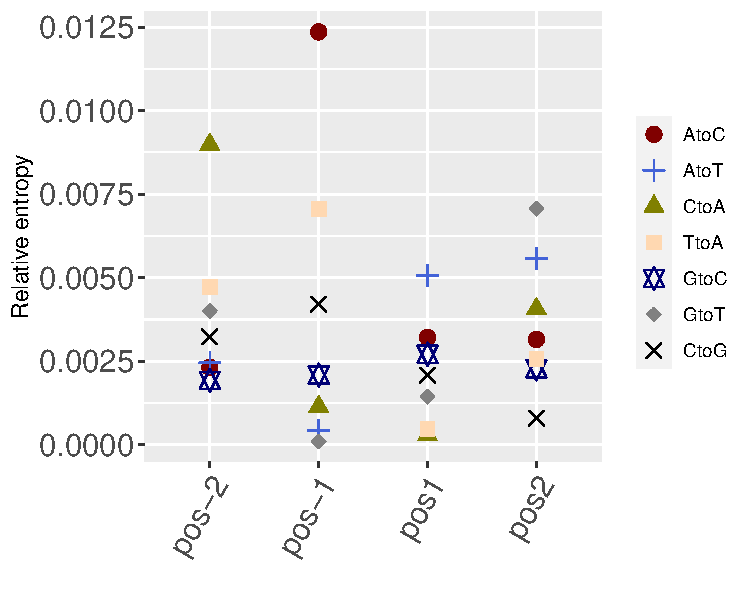
\includegraphics[scale=0.63]{graphics/nbr_transversion_Lymph-CLL.pdf}
    \caption{transversion/Lymph-CLL}
    \label{fig:transversion_lymph-cll}
    \end{subfigure} \\
    \vspace{0.5cm}
    
    \begin{subfigure}{.5\textwidth}
    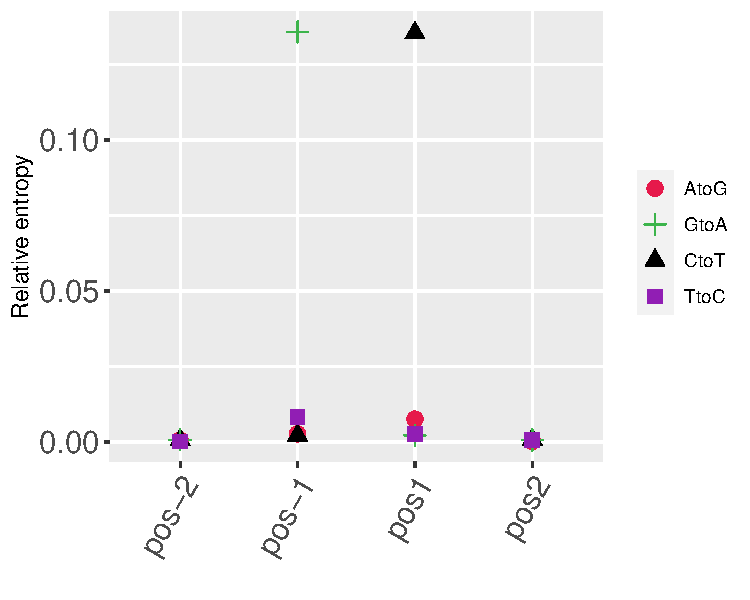
\includegraphics[scale=0.63]{graphics/nbr_transitions_Panc-AdenoCA.pdf}
    \caption{transitions/Panc-AdenoCA}
    \label{fig:transitions_panc-adenoca}
    \end{subfigure}
    ~
    \begin{subfigure}{.5\textwidth}
    \includegraphics[scale=0.63]{graphics/nbr_transversion_Panc-AdenoCA.pdf}
    \caption{transversion/Panc-AdenoCA}
    \label{fig:transversion_panc-adenoca}
    \end{subfigure} \\
    
    \begin{subfigure}{.5\textwidth}
    \includegraphics[scale=0.63]{graphics/nbr_transitions_Panc-Endocrine.pdf}
    \caption{transitions/Panc-Endocrine}
    \label{fig:transitions_panc-endocrine}
    \end{subfigure}
    ~
    \begin{subfigure}{.5\textwidth}
    \includegraphics[scale=0.63]{graphics/nbr_transversion_Panc-Endocrine.pdf}
    \caption{transversion/Panc-Endocrine}
    \label{fig:transversion_panc-endocrine}
    \end{subfigure} \\
    \caption{\textbf{Flanking bases are a good source of information.} Here, $RE$'s are shown the transitions and transversions for 10 cancers. This is an extension of Figure \ref{fig:nbr}. For each panel, each dot was derived from a pair of GLM. The x-axis is the flanking positions with respect to the substitution (substitution at 0); the y-axis is the $RE$ values. Continued on next page}
\end{figure}
\begin{figure}[ht!]\ContinuedFloat
    \begin{subfigure}{.5\textwidth}
    \includegraphics[scale=0.63]{graphics/nbr_transitions_Prost-AdenoCA.pdf}
    \caption{transitions/Prost-AdenoCA}
    \label{fig:transitions_prost-adenoca}
    \end{subfigure}
    ~
    \begin{subfigure}{.5\textwidth}
    \includegraphics[scale=0.63]{graphics/nbr_transversion_Prost-AdenoCA.pdf}
    \caption{transversion/Prost-AdenoCA}
    \label{fig:transversion_prost-adenoca}
    \end{subfigure} \\
    \vspace{0.5cm}
    \caption{\textbf{Flanking bases are a good source of information.} Here, $RE$'s are shown the transitions and transversions for 10 cancers. This is an extension of Figure \ref{fig:nbr}. For each panel, each dot was derived from a pair of GLM. The x-axis is the flanking positions with respect to the substitution (substitution at 0); the y-axis is the $RE$ values.}
    \label{fig:apdx_nbr}
\end{figure}